\documentclass[11pt,a4paper]{article}

\usepackage[T1]{fontenc}
\usepackage{lmodern}
\usepackage[margin=2.4cm]{geometry}
\usepackage{microtype}
\usepackage{amsmath,amssymb}
\usepackage{booktabs,array,multirow}
\usepackage{graphicx}
\usepackage{subcaption}
\usepackage{float}
\usepackage[font=small,labelfont=bf,skip=4pt]{caption}
\usepackage{xcolor}
\usepackage{fancyhdr}
\usepackage[hidelinks,pdfusetitle]{hyperref}
\usepackage{enumitem}
\usepackage{setspace}
\usepackage{url}

\definecolor{mlpblue}{HTML}{1F4E79}
\definecolor{lstmorange}{HTML}{C55A11}
\setlist{itemsep=2pt,topsep=4pt}
\setstretch{1.08}
\captionsetup{justification=centering}
\renewcommand{\arraystretch}{1.12}

\pagestyle{fancy}
\fancyhf{}
\lhead{\small TokaMark \texttt{task\_1-3}: CNN+MLP vs CNN+LSTM}
\rhead{\small Results report}
\cfoot{\small\thepage}
\renewcommand{\headrulewidth}{0.3pt}

\newcommand{\TrainTable}{%
CNN+MLP, plain baseline$^{a}$ & 3\,500 / 44 & 154.9 & 0.8723 & 0.1419 & 0.00389 \\
CNN+MLP, failure-aware (step loop) & 4\,200 / 53 & 194.4 & 0.8883 & 0.1590 & 0.00396 \\
CNN+MLP, failure-aware (epoch loop)$^{b}$ & 4\,056 / 52 & 198.2 & 0.9025 & 0.1512 & 0.00418 \\
CNN+LSTM, failure-aware (step loop) & 4\,200 / 53 & 190.2 & 0.9198 & 0.1680 & 0.00511 \\
}
\newcommand{\CleanTable}{%
CNN+MLP & 0.1514 $\pm$ 0.1215 & 0.0762 & 0.00832 & 0.00419 & 3\,450 \\
CNN+LSTM & 0.1681 $\pm$ 0.1036 & 0.0930 & 0.00923 & 0.00511 & 3\,450 \\
}
\newcommand{\RSTable}{%
Random dropout & 2.247 & 0.07 & 0.878 & 0.19 \\
Temporal gap & 0.904 & 0.17 & 0.615 & 0.27 \\
Disruption-proximate & 0.486 & 0.31 & 0.449 & 0.37 \\
Channel ablation & 0.341 & 0.44 & 0.316 & 0.53 \\
Group failure & 0.263 & 0.58 & 0.262 & 0.64 \\
Category ablation & 0.176 & 0.86 & 0.186 & 0.90 \\
}
\newcommand{\SweepTable}{%
\texttt{category\_abl|active\_coils} & 0.1549 & 0.1699 & 0.978 & 0.989 \\
\texttt{category\_abl|flux\_loop} & 0.1560 & 0.1762 & 0.970 & 0.954 \\
\texttt{category\_abl|pickup\_fields} & 0.1757 & 0.1858 & 0.862 & 0.905 \\
\texttt{category\_abl|plasma\_current} & 0.1530 & 0.1754 & 0.990 & 0.958 \\
\texttt{category\_abl|saddle\_voltage} & 0.1440 & 0.1629 & 1.052 & 1.032 \\
\texttt{category\_abl|solenoid} & 0.1563 & 0.1680 & 0.969 & 1.000 \\
\texttt{channel\_ablation|1} & 0.1602 & 0.1760 & 0.945 & 0.955 \\
\texttt{channel\_ablation|3} & 0.1928 & 0.2024 & 0.785 & 0.830 \\
\texttt{channel\_ablation|6} & 0.3415 & 0.3158 & 0.443 & 0.532 \\
\texttt{disruption\_proximate|0.1} & 0.2305 & 0.2090 & 0.657 & 0.804 \\
\texttt{disruption\_proximate|0.25} & 0.2553 & 0.2135 & 0.593 & 0.787 \\
\texttt{disruption\_proximate|0.5} & 0.4859 & 0.4488 & 0.312 & 0.375 \\
\texttt{group\_failure|magnetic\_probes} & 0.1757 & 0.1858 & 0.862 & 0.905 \\
\texttt{group\_failure|magnetics\_all} & 0.2626 & 0.2624 & 0.576 & 0.641 \\
\texttt{group\_failure|power\_supply} & 0.1573 & 0.1704 & 0.962 & 0.987 \\
\texttt{random\_dropout|0.1} & 0.9365 & 0.3602 & 0.162 & 0.467 \\
\texttt{random\_dropout|0.25} & 1.5495 & 0.6125 & 0.098 & 0.274 \\
\texttt{random\_dropout|0.5} & 2.2473 & 0.8776 & 0.067 & 0.192 \\
\texttt{temporal\_gap|0.2} & 0.4577 & 0.2809 & 0.331 & 0.598 \\
\texttt{temporal\_gap|0.4} & 0.5966 & 0.4100 & 0.254 & 0.410 \\
\texttt{temporal\_gap|0.6} & 0.9039 & 0.6147 & 0.167 & 0.273 \\
}
\newcommand{\ImputeTable}{%
Random dropout & CNN+MLP & 2.247 & 2.244 & 3.739 \\
 & CNN+LSTM & 0.878 & 0.922 & 0.609 \\
\midrule
Temporal gap & CNN+MLP & 0.904 & 0.849 & 1.718 \\
 & CNN+LSTM & 0.615 & 0.598 & 0.594 \\
\midrule
Disruption-proximate & CNN+MLP & 0.486 & 0.486 & 0.382 \\
 & CNN+LSTM & 0.449 & 0.449 & 0.312 \\
\midrule
Channel ablation & CNN+MLP & 0.341 & 0.431 & 0.459 \\
 & CNN+LSTM & 0.316 & 0.421 & 0.444 \\
\midrule
Group failure & CNN+MLP & 0.263 & 0.263 & 0.263 \\
 & CNN+LSTM & 0.262 & 0.262 & 0.262 \\
\midrule
Category ablation & CNN+MLP & 0.176 & 0.176 & 0.176 \\
 & CNN+LSTM & 0.186 & 0.186 & 0.186 \\
}
\newcommand{\PhysTable}{%
Clean & CNN+MLP & 3.48 & 17.8 & 16.2 & 62.2 & 25.0 & 0.0 \\
 & CNN+LSTM & 4.87 & 22.1 & 10.1 & 60.0 & 25.0 & 0.0 \\
\midrule
6 channels lost & CNN+MLP & 10.71 & 33.2 & 15.7 & 65.7 & 25.0 & 3.7 \\
 & CNN+LSTM & 8.64 & 28.7 & 16.2 & 63.6 & 25.0 & 7.4 \\
\midrule
Magnetics group lost & CNN+MLP & 7.65 & 29.9 & 15.4 & 56.3 & 25.0 & 0.0 \\
 & CNN+LSTM & 8.38 & 31.2 & 15.2 & 56.4 & 25.0 & 0.0 \\
\midrule
Temporal gap 40\% & CNN+MLP & 13.49 & 43.5 & 36.4 & 62.7 & 25.0 & 55.6 \\
 & CNN+LSTM & 11.62 & 37.2 & 22.9 & 75.7 & 25.0 & 25.9 \\
\midrule
Pre-disruption 25\% & CNN+MLP & 8.29 & 34.1 & 25.6 & 67.0 & 12.5 & 0.0 \\
 & CNN+LSTM & 8.21 & 30.3 & 22.0 & 60.3 & 50.0 & 7.4 \\
\midrule
Random dropout 10\% & CNN+MLP & 11.54 & 41.8 & 27.5 & 70.8 & 50.0 & 3.7 \\
 & CNN+LSTM & 8.49 & 28.8 & 13.8 & 59.8 & 25.0 & 11.1 \\
}
\newcommand{\CritTable}{%
\texttt{flux\_loop} & 15 & 4.12 & +0.64 & 6.44 & +1.57 \\
\texttt{ccbv} & 40 & 3.32 & -0.15 & 4.71 & -0.16 \\
\texttt{obr} & 18 & 3.86 & +0.38 & 5.14 & +0.27 \\
\texttt{obv} & 18 & 3.62 & +0.15 & 4.95 & +0.09 \\
\texttt{saddle\_v} & 12 & 3.57 & +0.09 & 4.79 & -0.08 \\
\texttt{coil\_i} & 10 & 3.37 & -0.11 & 6.12 & +1.26 \\
\texttt{solenoid\_i} & 1 & 3.57 & +0.09 & 5.96 & +1.09 \\
\texttt{ip} & 1 & 3.24 & -0.24 & 5.52 & +0.65 \\
}
\newcommand{\CleanBndMLP}{3.48}
\newcommand{\CleanBndLSTM}{4.87}
\newcommand{\MitTable}{%
CNN+MLP & clean & 3.48 & 4.99 & 25 / 100 / 100 & 0 / 0 / 0 & 18.8 \\
 & spike & 23.18 & 4.93 & 75 / 100 / 100 & 26 / 0 / 0 & 18.5 \\
 & redundant probe dead & 4.52 & 6.15 & 50 / 100 / 100 & 0 / 0 / 0 & 18.6 \\
 & critical branch dead & 8.74 & 6.15 & 12 / 100 / 100 & 15 / 0 / 0 & 18.9 \\
 & group loss & 12.69 & 7.93 & 12 / 100 / 100 & 30 / 0 / 0 & 18.5 \\
 & 6 channels lost & 12.88 & 14.69 & 0 / 100 / 100 & 81 / 0 / 0 & 18.6 \\
 & gap 40\% & 12.35 & 4.32 & 25 / 100 / 100 & 30 / 0 / 0 & 21.4 \\
 & pre-disr. 25\% & 11.21 & 4.37 & 50 / 100 / 100 & 11 / 0 / 0 & 20.3 \\
\midrule
CNN+LSTM & clean & 4.87 & 6.57 & 25 / 100 / 100 & 0 / 0 / 0 & 19.6 \\
 & spike & 14.25 & 6.56 & 50 / 100 / 100 & 37 / 0 / 0 & 20.3 \\
 & redundant probe dead & 5.68 & 7.65 & 12 / 100 / 100 & 0 / 0 / 0 & 19.2 \\
 & critical branch dead & 8.59 & 7.65 & 12 / 100 / 100 & 4 / 0 / 0 & 18.9 \\
 & group loss & 11.79 & 8.55 & 12 / 100 / 100 & 30 / 0 / 0 & 19.5 \\
 & 6 channels lost & 15.95 & 15.34 & 12 / 100 / 100 & 48 / 0 / 0 & 18.4 \\
 & gap 40\% & 10.69 & 6.67 & 38 / 100 / 100 & 19 / 0 / 0 & 20.9 \\
 & pre-disr. 25\% & 15.59 & 6.69 & 75 / 100 / 100 & 4 / 0 / 0 & 20.7 \\
}
\newcommand{\DeltaMLP}{88.4}
\newcommand{\LatMLP}{19.2}
\newcommand{\NcalMLP}{792}
\newcommand{\DeltaLSTM}{93.5}
\newcommand{\LatLSTM}{19.7}
\newcommand{\NcalLSTM}{792}
\newcommand{\NHazard}{27}
\newcommand{\NSafe}{8}
\newcommand{\NRMSEmlp}{0.1512}
\newcommand{\NRMSElstm}{0.1680}
\newcommand{\NRMSEmlpold}{0.1590}


\newcommand{\psihat}{\hat{\psi}}
\newcommand{\mlp}{\textcolor{mlpblue}{\textbf{CNN+MLP}}}
\newcommand{\lstm}{\textcolor{lstmorange}{\textbf{CNN+LSTM}}}

\begin{document}

% ------------------------------------------------------------------ title
\begin{titlepage}
\centering
\vspace*{2.2cm}
{\large Deep Learning End-Semester Project --- Team 15\par}
\vspace{1.2cm}
{\Huge\bfseries Failure-Resilient, Physics-Informed\\[4pt] Plasma Equilibrium Reconstruction\par}
\vspace{0.6cm}
{\Large TokaMark \texttt{task\_1-3} on MAST\par}
\vspace{1.4cm}
{\LARGE Results of the CNN+MLP and CNN+LSTM Pipelines\\[4pt] across the Four Novel Modules\par}
\vspace{2.4cm}
\begin{tabular}{rl}
\textbf{Task} & 2D poloidal-flux ($\psi$) reconstruction, $65\times65$ grid\\
\textbf{Models} & Failure-aware CNN+MLP and CNN+LSTM, flux-loop PINN loss\\
\textbf{Hardware} & Kaggle, 2$\times$ NVIDIA Tesla T4\\
\textbf{Evaluation} & 46 held-out test shots, 3\,450 windows (random split)\\
\end{tabular}
\vfill
{\large Every number in this report is read from the downloaded run artefacts by\\
\texttt{cnn\_mlp/report/build\_report\_assets.py}; nothing is typed in by hand.\par}
\vspace{1cm}
\end{titlepage}

\tableofcontents
\clearpage

% ------------------------------------------------------------------ summary
\section{Executive summary}
We trained and stress-tested two failure-aware reconstruction networks, \mlp{} and \lstm{}, which map 115 magnetic and
machine-state probes (eight sensor branches) to the 2D poloidal flux $\psi$ inside the MAST vessel. Both use the same
mask-gated architecture, the same structured failure augmentation, the same 15 flux-loop physics loss, the same
shots and the same optimiser settings. The main findings are:

\begin{enumerate}
  \item \textbf{Clean accuracy favours the MLP.} Test NRMSE is \NRMSEmlpold{} for the step-trained MLP, \NRMSElstm{} for the LSTM
        ($+5.7\%$) and \NRMSEmlp{} for a newer, epoch-trained MLP. The LSTM's mean absolute error is 29\% higher than the MLP's
        (0.00511 vs 0.00396\,Wb).
  \item \textbf{The LSTM degrades far more gracefully under partial sensor damage.} At 10\% random dropout the LSTM's NRMSE is
        0.36 against 0.94 for the MLP; for a 40\% temporal gap it is 0.41 against 0.60. Both models handle the loss of a whole
        sensor group about equally well, because the health mask makes that case explicit.
  \item \textbf{Module 1 (physics metrics)} converts these errors to centimetres: the plasma boundary is off by
        \CleanBndMLP\,cm (MLP) and \CleanBndLSTM\,cm (LSTM) on healthy input and by roughly 8--13\,cm under failures.
        X-point and wall-clearance metrics are not reliable on this data (Section~\ref{sec:m1}).
  \item \textbf{Module 3 (minimal sensor set) prunes nothing.} The clean boundary error already exceeds the 2\,cm tolerance, so
        all 115 probes are retained for both models.
  \item \textbf{Module 4 (adaptive mitigation) helps on some faults but does not meet its design targets.} It reduces
        boundary error on spikes, gaps and pre-disruption windows, but its conformal margin ($\approx$80--94\,cm) flags every
        window, and its loop latency ($\approx$19--20\,ms) exceeds the 5\,ms control-loop budget.
\end{enumerate}

\noindent\textbf{Reading guide.} Sections~\ref{sec:setup}--\ref{sec:m2} describe the setup and the trained models (Module~2),
Section~\ref{sec:m1} defines the physics layer (Module~1), Section~\ref{sec:robust} reports the sensor-failure sweep that drives
Modules~3 and~4 (Sections~\ref{sec:m3} and~\ref{sec:m4}), and Section~\ref{sec:limits} lists the limitations that should accompany
any number quoted from this report.

% ------------------------------------------------------------------ setup
\section{Experimental setup}\label{sec:setup}

\subsection{Task and data}
TokaMark \texttt{task\_1-3} asks a network to reconstruct the poloidal flux $\psi(R,Z)$ on a $65\times65$ grid
($R\in[0.2,2.0]$\,m, $Z\in[-1.5,1.5]$\,m, i.e.\ $\Delta R=2.8125$\,cm and $\Delta Z=4.6875$\,cm per pixel) from eight input branches: 15 flux
loops, 40+18+18 poloidal pickup probes (CCBV, OBR, OBV), 12 saddle-loop voltages, 10 active-coil currents, the solenoid
current and the plasma current. A budget-limited random subset of the official random split was used: 606 training, 74
validation and 60 test shots (46 test shots remain after the official outlier and EFIT-quality filters). Both models use the
\emph{same} shot selection.

\subsection{Identical training protocol}
\begin{table}[H]
\centering
\caption{Training configuration shared by both models. Only the recurrent backbone differs.}
\small
\begin{tabular}{@{}p{2.2cm}p{4.4cm}p{3.5cm}p{4.6cm}@{}}
\toprule
Optimiser & Adam, lr $10^{-4}$, wd $10^{-4}$ & Failure augmentation & $p=0.5$ \\
Batch size & 512 (drop last) & PINN weight $\lambda$ & 0.1 \\
Loss & MultiOutputMSELoss + PINN & Gradient clipping & 1.0 (norm) \\
Validation & every 100 steps & LR schedule & ReduceLROnPlateau (0.5, patience 3) \\
Early stopping & patience 10 validations & Seed & 23 \\
Data & 606 / 74 / 60 shots & Wall-clock limit & 7\,h \\
\bottomrule
\end{tabular}
\end{table}

The CNN+LSTM kernel was built from the CNN+MLP notebook with one change of model type; the CNN+MLP run's shot selection is
embedded so that data are identical, and \texttt{DataParallel} was forced over both T4 GPUs (the CNN+MLP run's automatic
benchmark chose a single GPU). Both kernels execute the same \texttt{pipeline.py}.

% ------------------------------------------------------------------ module 2
\section{Module 2: failure-aware architecture and flux-loop PINN}\label{sec:m2}

\subsection{Architecture}
Each of the eight sensor branches has its own CNN encoder. With health flags $m_i\in\{0,1\}$ the encoder output is gated,
$h_i^{\text{gated}}=h_i\,m_i$, and the flag vector is also fed to the backbone so that it knows \emph{which} inputs are missing:
\begin{align}
\text{MLP:}\quad & c=\mathrm{MLP}\big([h_1^{\text{gated}},\dots,h_8^{\text{gated}},\,m_1,\dots,m_8]\big),\\
\text{LSTM:}\quad & (e_t)_{t=1}^{W}=\mathrm{LSTM}\big([h_{1,t}^{\text{gated}},\dots,h_{8,t}^{\text{gated}},\,m_1,\dots,m_8]\big),
\end{align}
followed by the upstream decoder and CNN output head. For the LSTM the flags are appended to every timestep of the encoder
input. When no mask is supplied (evaluation of an unannotated input), an all-zero branch is treated as dead.

\subsection{Structured failure augmentation and physics loss}
During training, with probability $p=0.5$ a window is corrupted: 40\% of the time one to three random branches are zeroed,
30\% of the time a correlated cluster is zeroed (e.g.\ all pickup probes), and 30\% of the time one or two branches lose half
their time axis. The corresponding flags are set to $0$. The loss adds a boundary-consistency term at the 15 wall flux-loop
pixels $(R_k,Z_k)$:
\begin{equation}
\mathcal L=\mathcal L_{\text{MSE}}+\lambda\,\frac1K\sum_{k=1}^{15} m_{\mathrm{fl}}\,\big(\psihat(R_k,Z_k)-\psi(R_k,Z_k)\big)^2,\qquad \lambda=0.1,
\end{equation}
where $m_{\mathrm{fl}}$ is the health flag of the flux-loop branch (a dead sensor cannot anchor the boundary).

\subsection{Training results and clean accuracy}
\begin{table}[H]
\centering
\caption{Training outcome and test accuracy (official evaluator, 46 test shots, un-standardised). $^{a}$From the earlier plain baseline
run; not failure-aware. $^{b}$A later run with epoch-based validation (patience 20 epochs); its loop therefore differs from the
other failure-aware runs, so differences to the LSTM are indicative rather than controlled.}
\label{tab:train}
\small
\begin{tabular}{@{}lrrrcc@{}}
\toprule
Model & Steps / epochs & Minutes & Best val & NRMSE & MAE (Wb) \\
\midrule
\TrainTable
\bottomrule
\end{tabular}
\end{table}

\begin{table}[H]
\centering
\caption{Clean test metrics from the robustness engine (same protocol as the sweep; agree with Table~\ref{tab:train} to three decimals).}
\small
\begin{tabular}{@{}lccccr@{}}
\toprule
Model & NRMSE & NMAE & RMSE (Wb) & MAE (Wb) & Windows \\
\midrule
\CleanTable
\bottomrule
\end{tabular}
\end{table}

\paragraph{Observations.} (i) Against the like-for-like step-trained MLP, the LSTM is 5.7\% worse in NRMSE and 29\% worse in MAE
and ends with a higher validation loss (0.920 vs 0.888). (ii) Both models overfit strongly: the training loss falls to
$\approx0.02$--$0.05$ while validation loss stays near 0.9, so the remaining error is a generalisation gap, not an optimisation
failure. (iii) The PINN term is active and decreases during training (Figure~\ref{fig:lstm-loss}). For the LSTM the five inner-wall
flux loops are fitted well (about 0.002\,Wb, below the grid-wide mean of 0.005\,Wb), while the ten outer-wall loops sit around or slightly
above the grid-wide level (Figure~\ref{fig:lstm-diag}, read from the plot).

\begin{figure}[H]
\centering
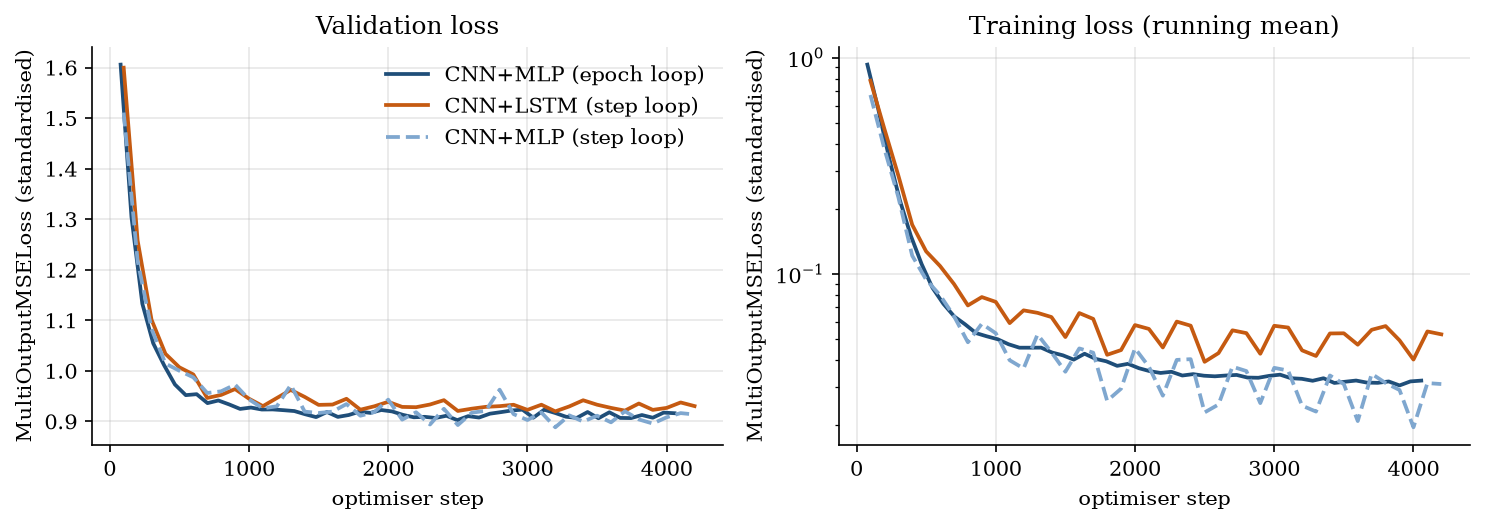
\includegraphics[width=\textwidth]{figures/cmp_training.png}
\caption{Validation (left) and training (right) loss of the three failure-aware runs. All stop by the early-stopping rule.}
\label{fig:cmp-train}
\end{figure}

\begin{figure}[H]
\centering
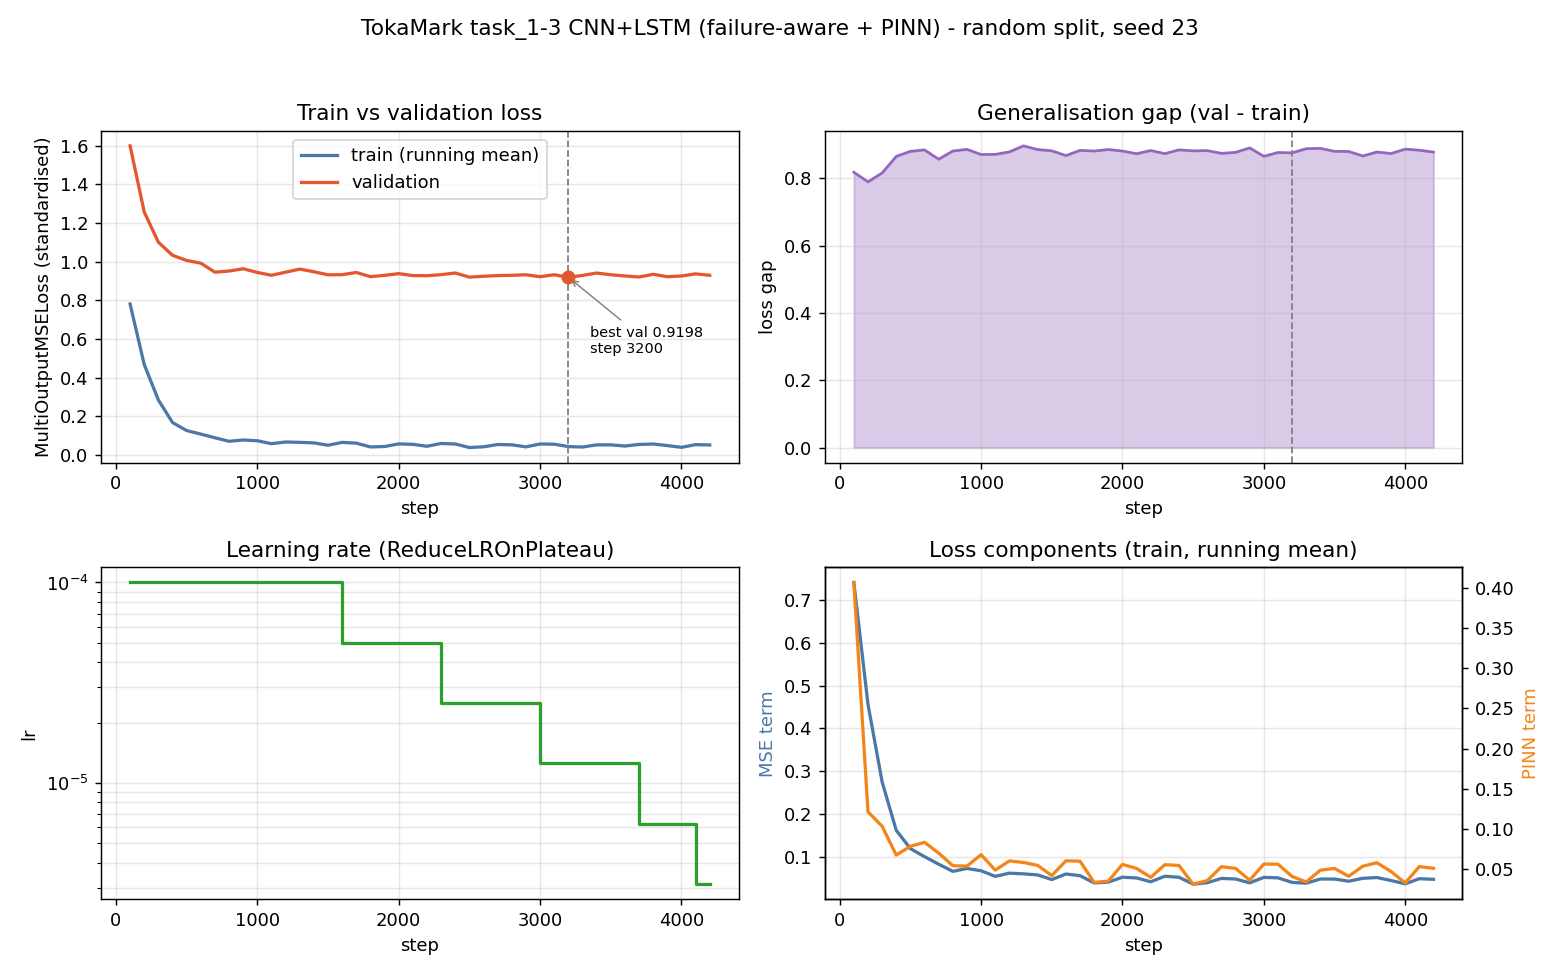
\includegraphics[width=0.93\textwidth]{figures/lstm_loss_curves.png}
\caption{\lstm{} training dashboard: train/validation loss, generalisation gap, learning-rate schedule, and the MSE and flux-loop PINN terms.}
\label{fig:lstm-loss}
\end{figure}

\begin{figure}[H]
\centering
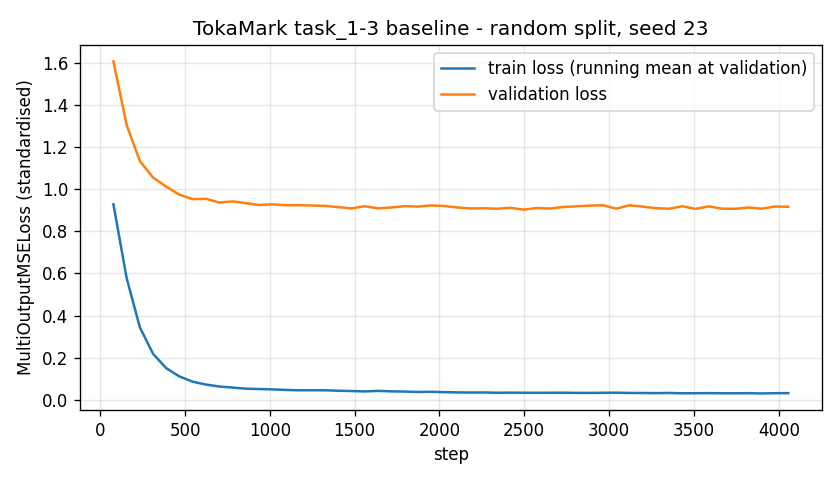
\includegraphics[width=0.93\textwidth]{figures/mlp_loss_curves.png}
\caption{\mlp{} (epoch-loop run) training curves, as produced by the pipeline.}
\end{figure}

\subsection{Reconstruction quality}
\begin{figure}[H]
\centering
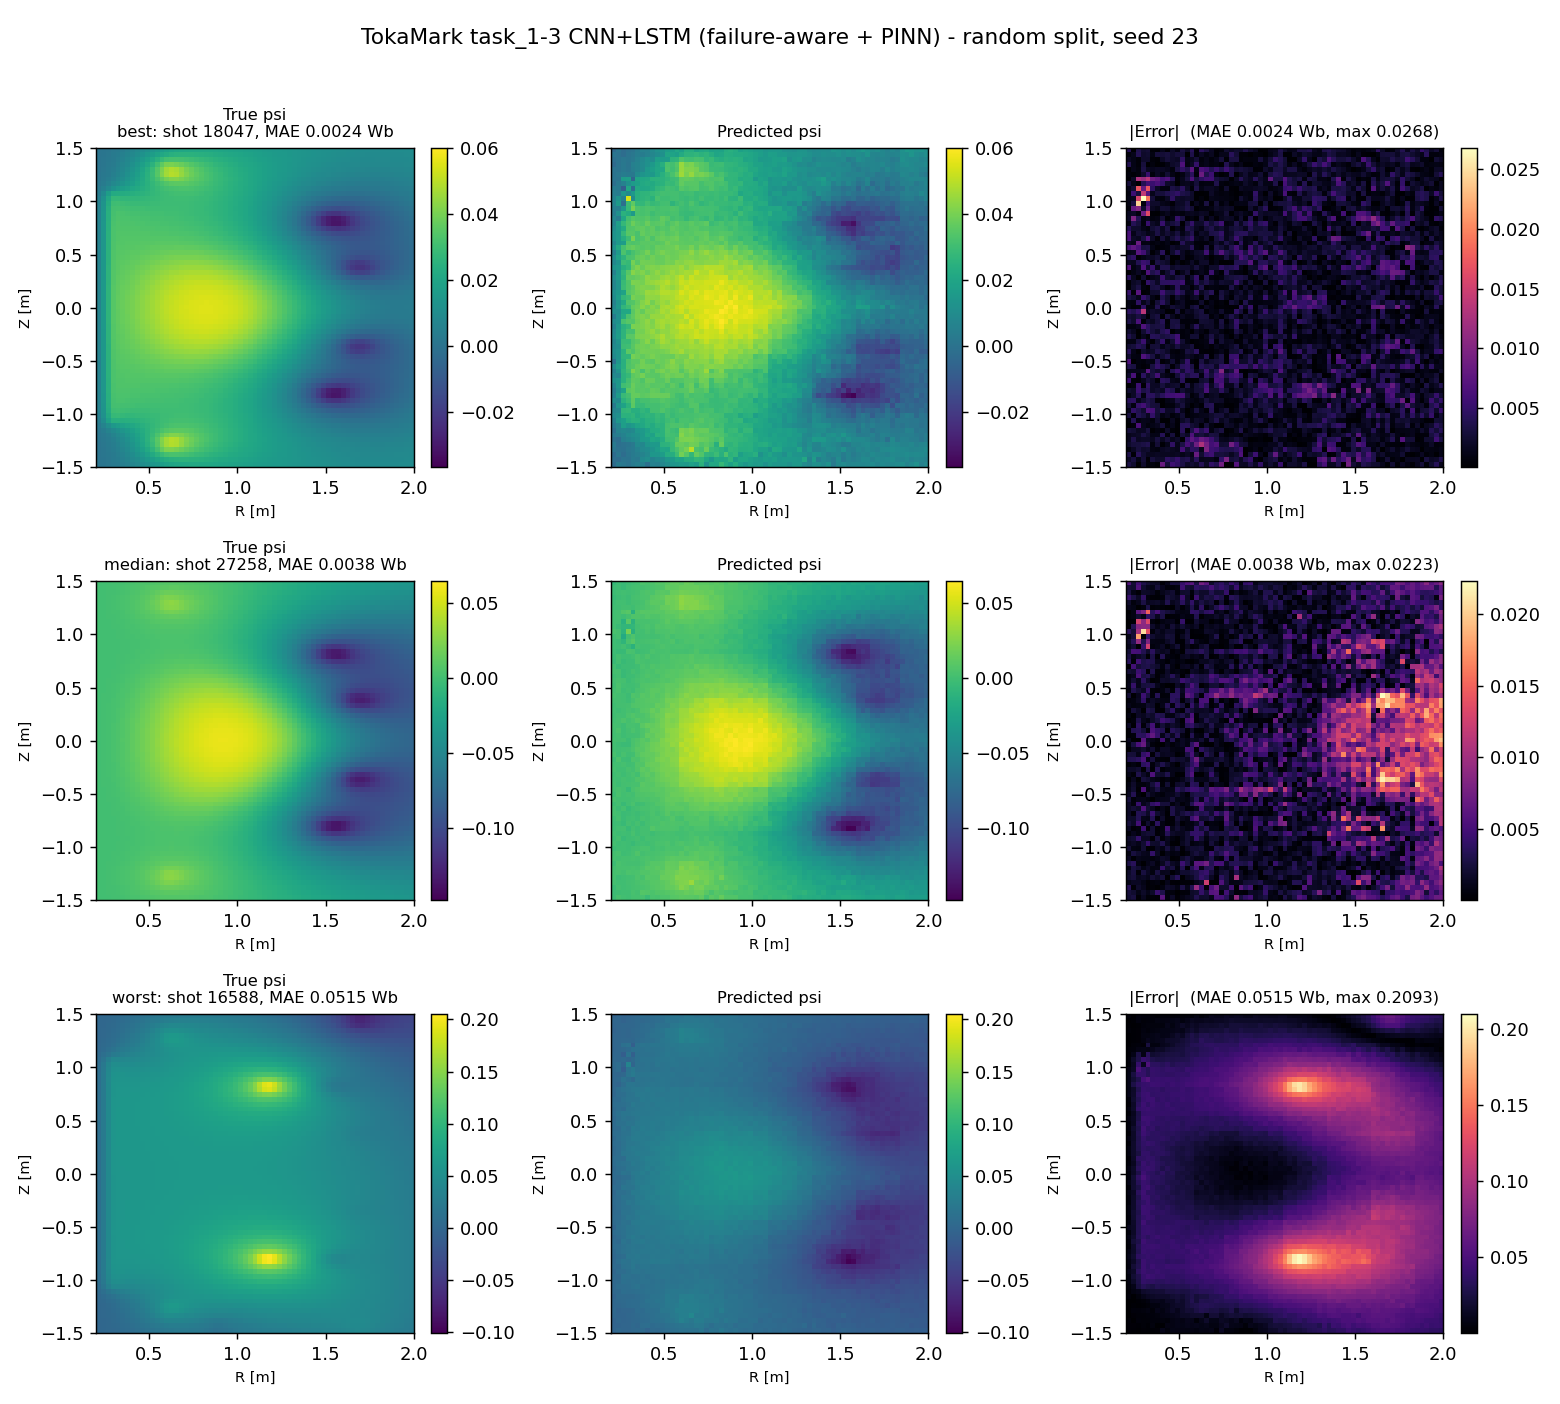
\includegraphics[width=\textwidth]{figures/lstm_psi_reconstruction_samples.png}
\caption{\lstm{}: true $\psi$, prediction and absolute error for the best, median and worst window of the first test batch.}
\label{fig:lstm-psi}
\end{figure}

\begin{figure}[H]
\centering
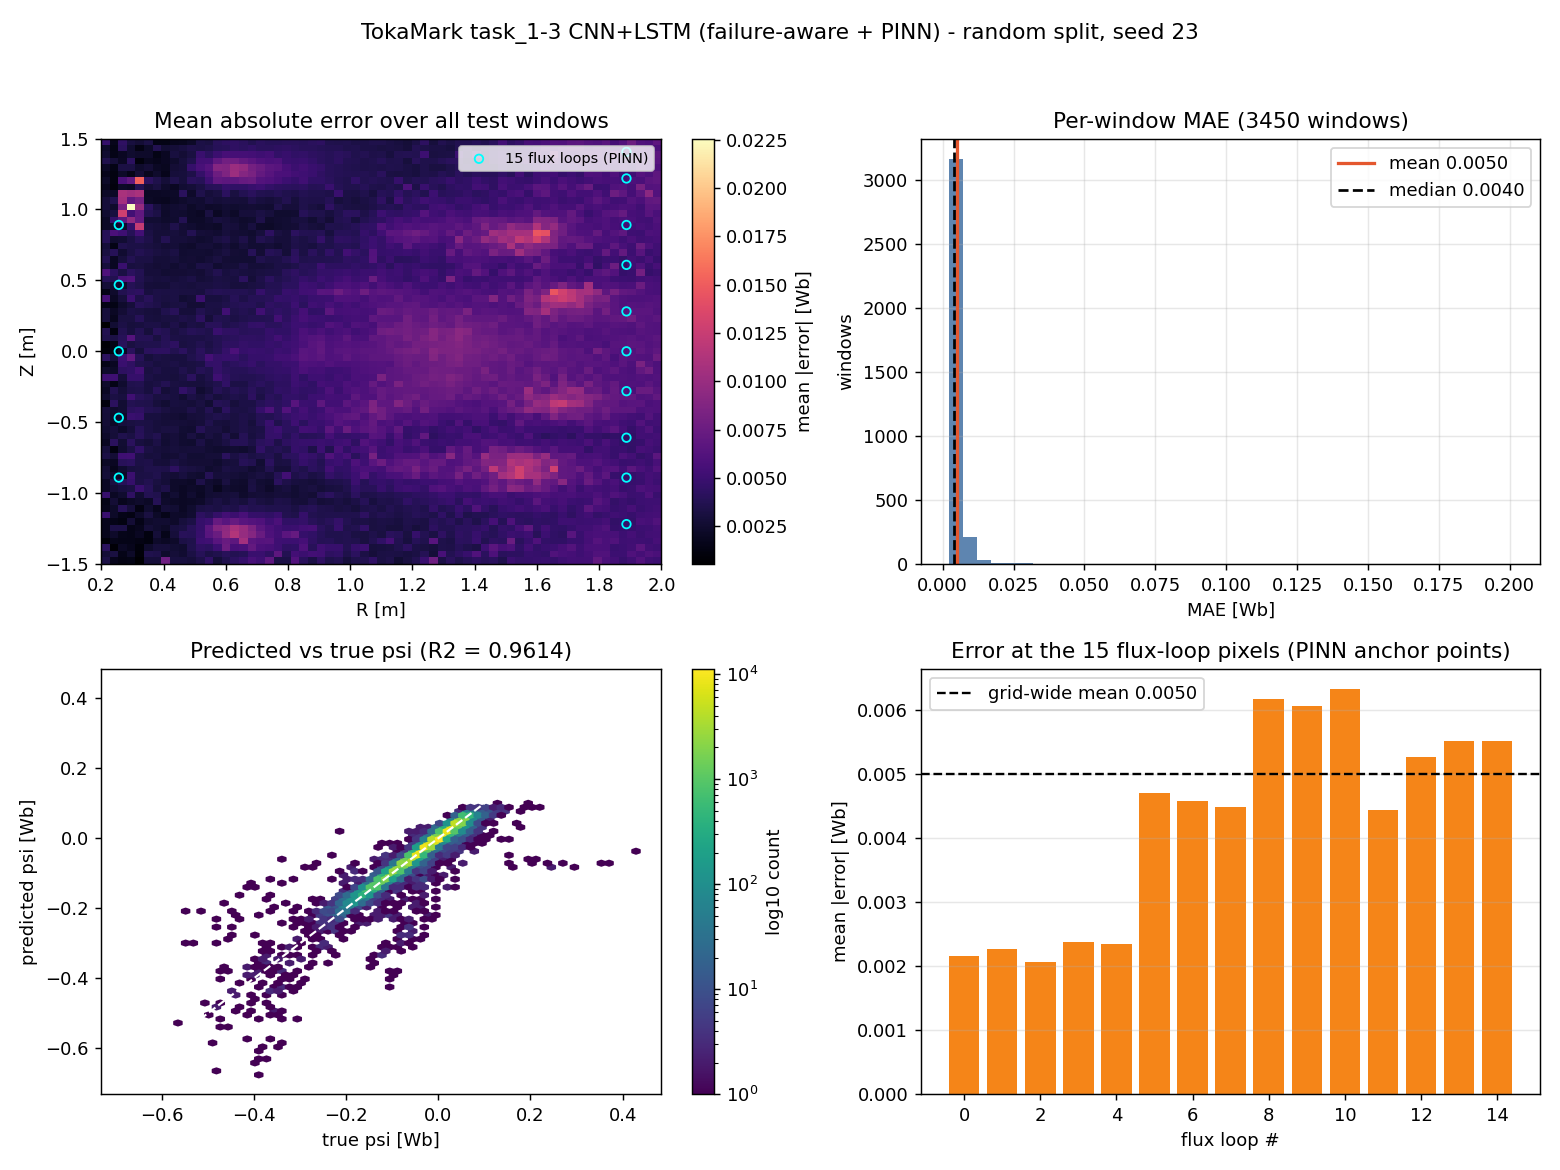
\includegraphics[width=\textwidth]{figures/lstm_test_error_diagnostics.png}
\caption{\lstm{} error diagnostics over all 3\,450 test windows: mean error map with the 15 flux loops (top left), per-window MAE
(top right), predicted vs true $\psi$ (bottom left; sparse outliers drive $R^2=0.96$) and the error at the flux-loop pixels (bottom right).}
\label{fig:lstm-diag}
\end{figure}

\begin{figure}[H]
\centering
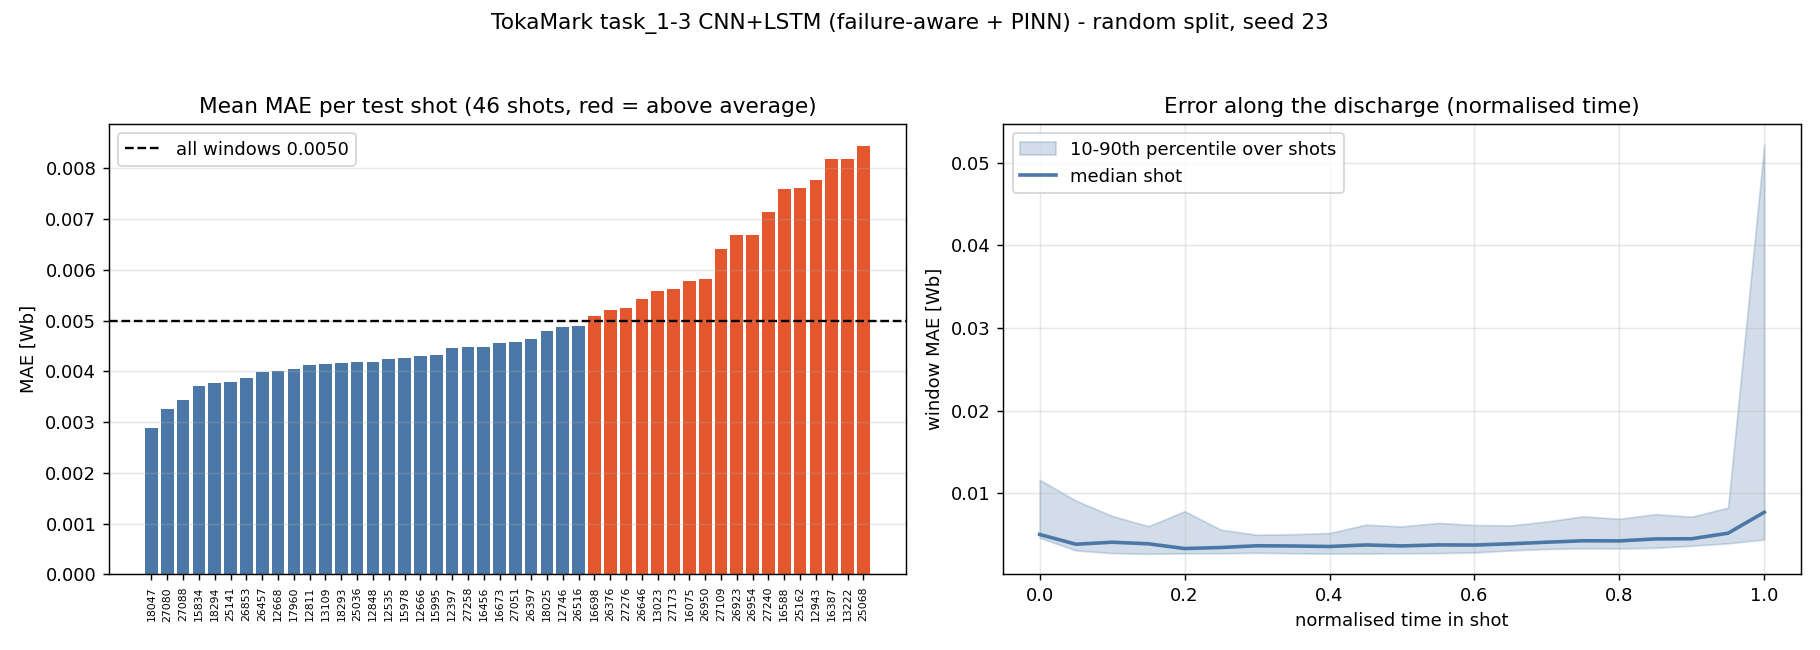
\includegraphics[width=\textwidth]{figures/lstm_per_shot_error.png}
\caption{\lstm{} error per test shot (left) and along the normalised discharge time (right). Error is concentrated in a few shots rather than uniform.}
\end{figure}

\begin{figure}[H]
\centering
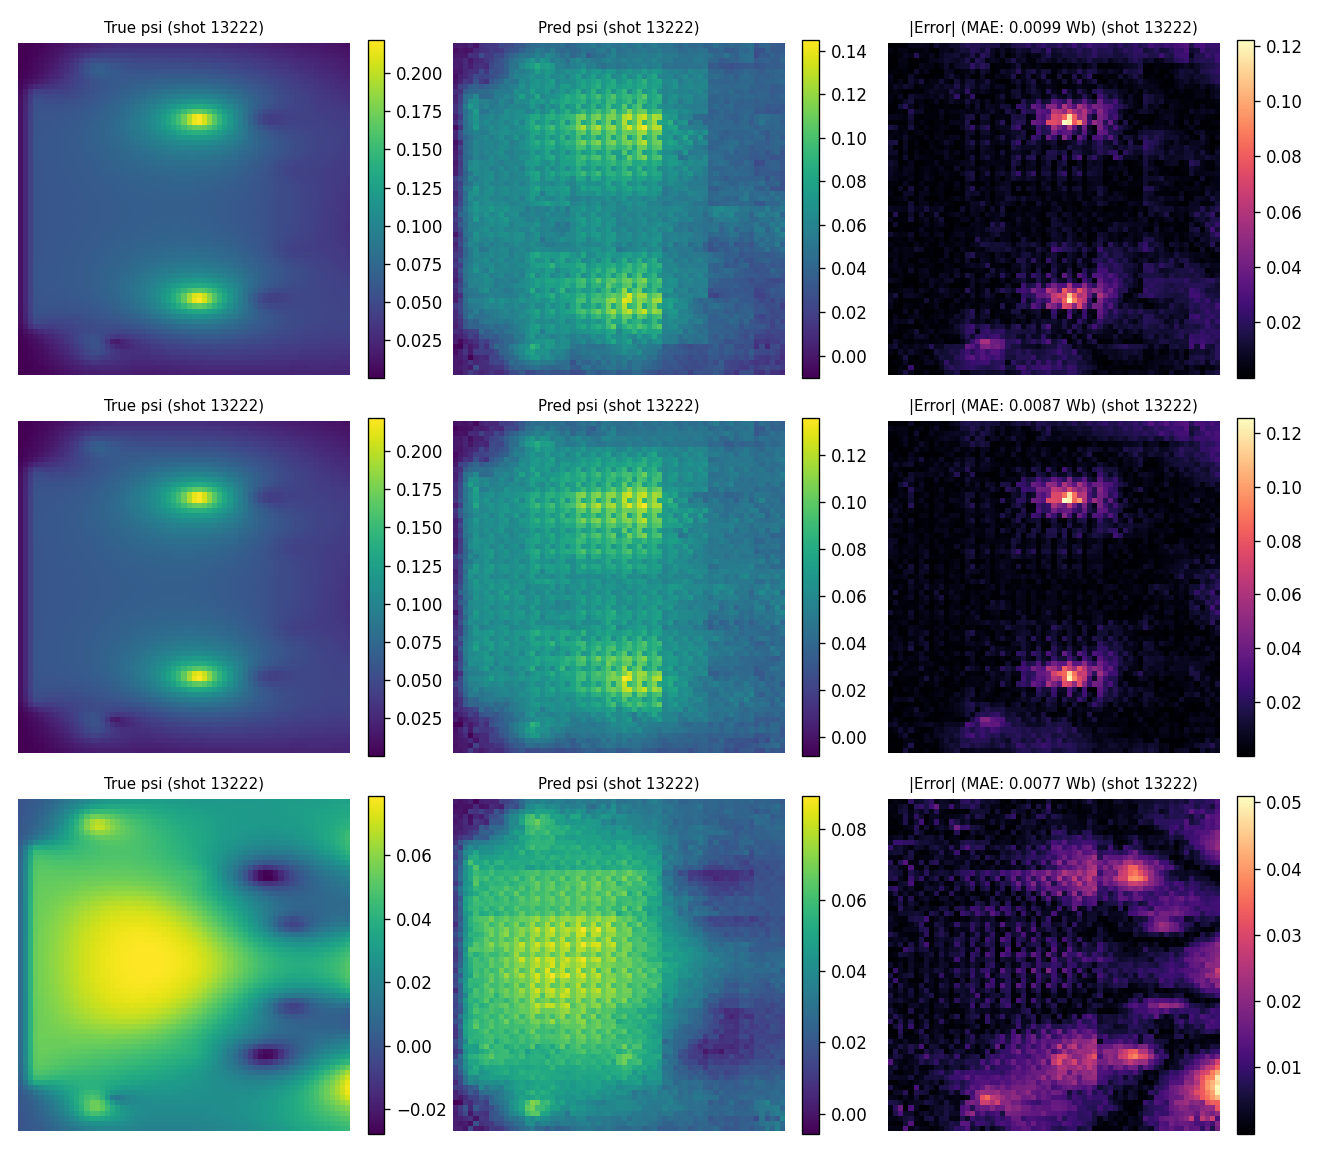
\includegraphics[width=\textwidth]{figures/mlp_psi_reconstruction_samples.png}
\caption{\mlp{} (epoch-loop run) reconstruction samples as produced by the pipeline (first three test windows).}
\end{figure}

% ------------------------------------------------------------------ module 1
\section{Module 1: physics-aware evaluation}\label{sec:m1}
NRMSE is dominated by cold vacuum pixels and hides small shifts of the last closed flux surface (LCFS). Module 1 therefore
converts the $65\times65$ predictions to centimetres using the grid scales of Section~\ref{sec:setup}:
\begin{itemize}
  \item \textbf{Boundary error.} The LCFS is the contour at $\psi_{\mathrm{LCFS}}=\psi_{\min}+0.35(\psi_{\max}-\psi_{\min})$ of the
        \emph{true} field. The predicted field is cut at that same level, so noise in the prediction does not move the level. We report the
        mean symmetric nearest-point distance between the two contours (and the Hausdorff distance).
  \item \textbf{Magnetic-axis shift}: distance between the true and predicted flux extremum (sub-pixel, same vertical half).
  \item \textbf{X-point error}: distance between saddle points where $\nabla\psi=0$ and $\det H<0$.
  \item \textbf{False / missed wall alarm}: clearance of the contour below 5\,cm. Clearance is the distance to the \emph{grid edge},
        a proxy for the vessel wall, because the true wall geometry is not part of the data.
\end{itemize}

\begin{table}[H]
\centering
\caption{Module 1 metrics (cm) on 35 test windows per pass; alarm rates in \%. Zero-fill corruption. ``Magnetics group lost'' zeroes all
three pickup-probe families.}
\label{tab:phys}
\small
\begin{tabular}{@{}llrrrrrr@{}}
\toprule
Pass & Model & Boundary & Hausdorff & Axis & X-point & False & Missed \\
\midrule
\PhysTable
\bottomrule
\end{tabular}
\end{table}

\begin{figure}[H]
\centering
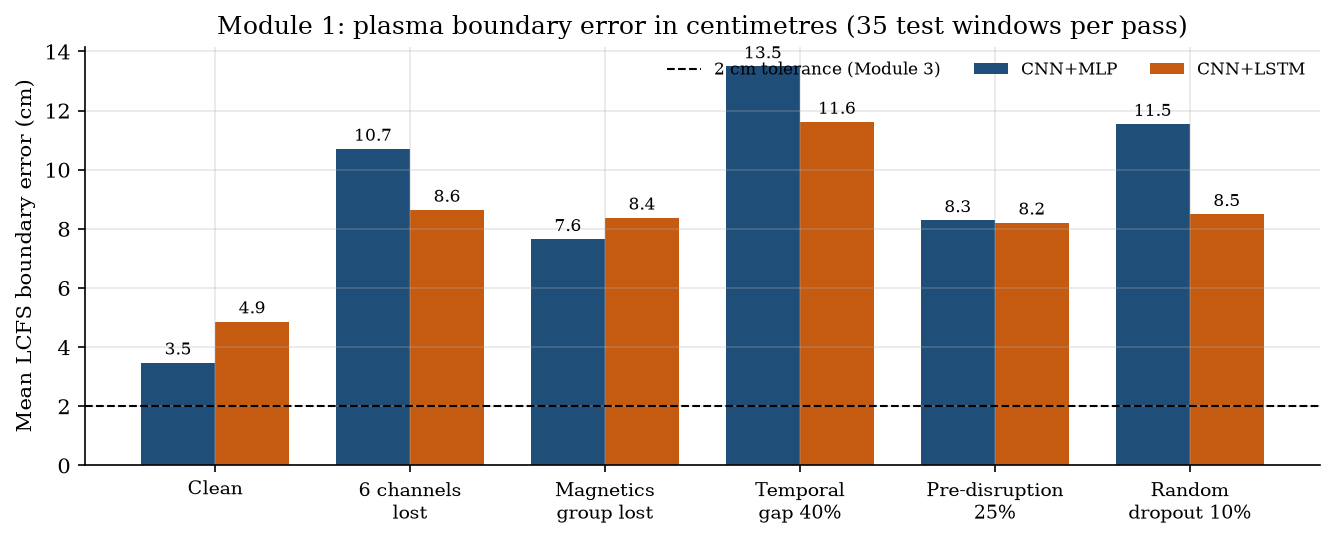
\includegraphics[width=0.85\textwidth]{figures/cmp_boundary_cm.png}
\caption{Mean LCFS boundary error in centimetres. The 2\,cm line is the tolerance used by Module 3.}
\label{fig:bnd}
\end{figure}

\paragraph{Interpretation.} On healthy input the MLP places the boundary more accurately (\CleanBndMLP{} vs \CleanBndLSTM\,cm),
consistent with its lower NRMSE. Under every failure pass the errors grow to roughly 8--13\,cm, and the LSTM is closer than the MLP
on 6-channel loss, temporal gaps and random dropout, while the MLP is slightly better for magnetics-group loss. \textbf{Caveats:}
(a) each point rests on 35 windows, so differences of 1--2\,cm are within noise; (b) the X-point error is $\approx$60\,cm even on clean
input and is not meaningful; (c) because the clearance proxy is the grid edge, most windows (\NHazard{} of 35) count as ``hazard'', so the alarm
rates should not be quoted as safety performance.

% ------------------------------------------------------------------ robustness
\section{Sensor-failure robustness sweep}\label{sec:robust}
Both frozen checkpoints are evaluated on the 46 test shots under 63 corruption passes (21 settings $\times$ three imputation modes),
following Gupta et al.\ (arXiv 2607.11915): random dropout (severity 0.1/0.25/0.5), channel ablation (1/3/6 channels), category
ablation (six sensor categories), temporal gaps (severity 0.2/0.4/0.6), correlated group failure, and disruption-proximate corruption. The
\emph{robustness score} is $\mathrm{RS}=\mathrm{NRMSE}_{\text{clean}}/\mathrm{NRMSE}_{\text{corrupted}}$ for the worst setting of each
scenario ($1$ = no damage). Inference ran on two T4 GPUs.

\begin{table}[H]
\centering
\caption{Worst-case NRMSE and robustness score per scenario (zero-fill; the full list of 21 settings is in Appendix~\ref{app:sweep}).}
\label{tab:rs}
\small
\begin{tabular}{@{}lcccc@{}}
\toprule
 & \multicolumn{2}{c}{\mlp} & \multicolumn{2}{c}{\lstm} \\
\cmidrule(lr){2-3}\cmidrule(lr){4-5}
Scenario & NRMSE & RS & NRMSE & RS \\
\midrule
\RSTable
\bottomrule
\end{tabular}
\end{table}

\begin{figure}[H]
\centering
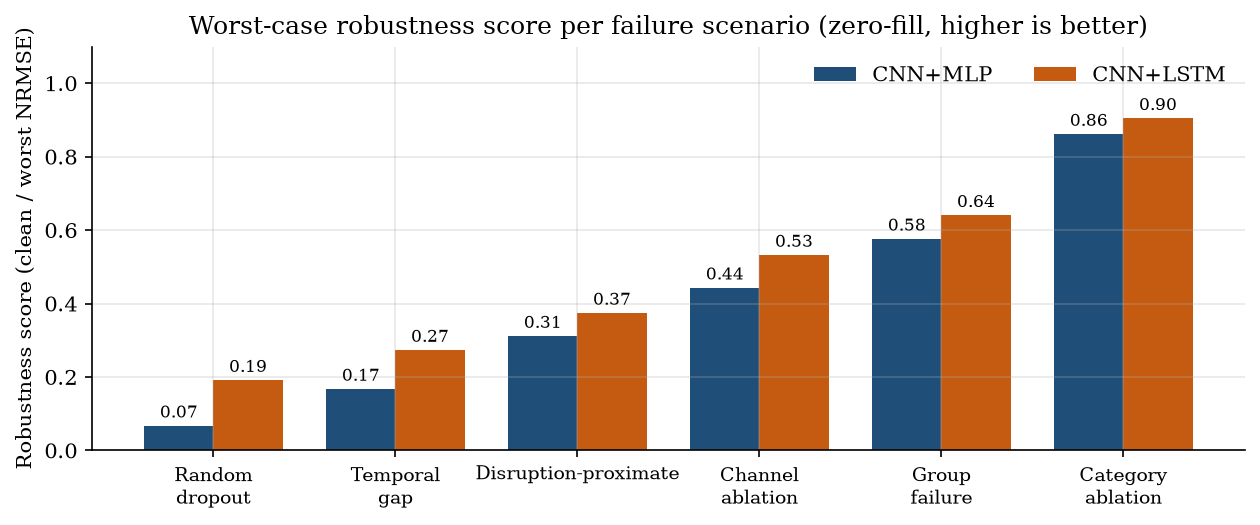
\includegraphics[width=0.85\textwidth]{figures/cmp_robustness_score.png}
\caption{Worst-case robustness score per failure scenario.}
\end{figure}

\begin{figure}[H]
\centering
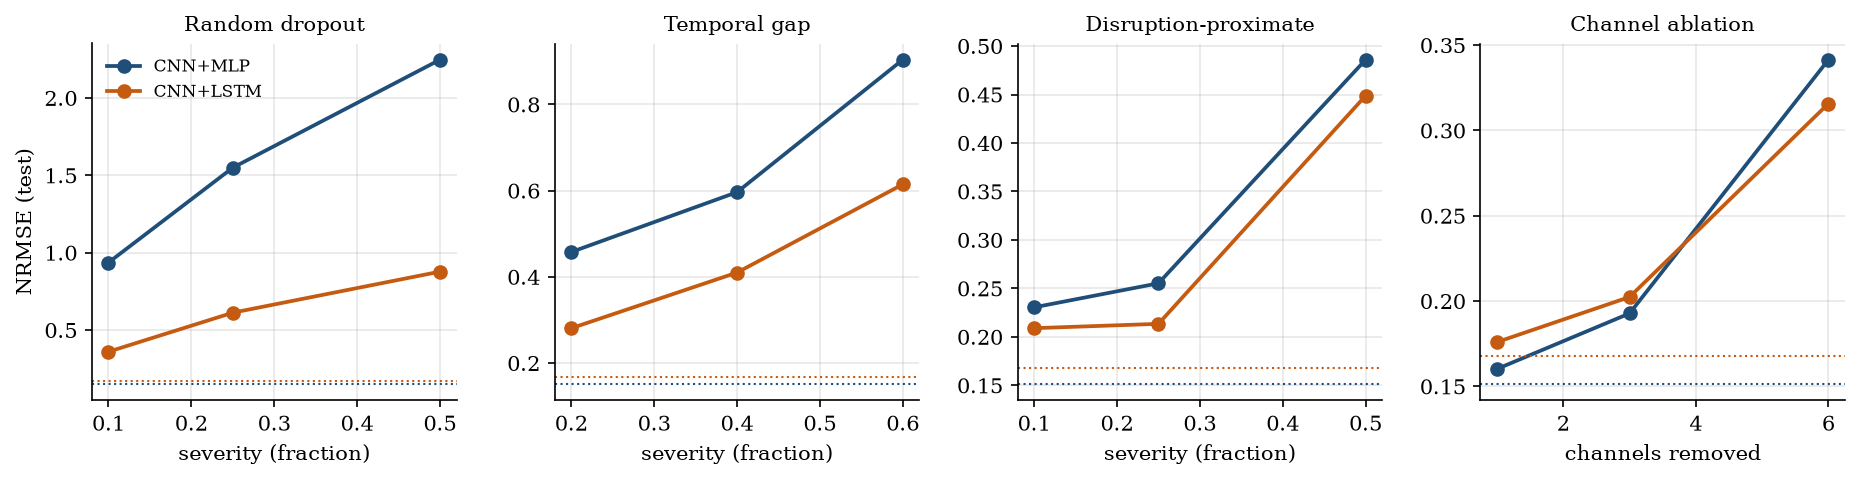
\includegraphics[width=\textwidth]{figures/cmp_degradation.png}
\caption{NRMSE as corruption severity increases (dotted lines: clean NRMSE). The MLP's error explodes with random dropout, while the LSTM's grows gradually.}
\end{figure}

\paragraph{Findings.}
\begin{itemize}
  \item \textbf{Whole-sensor loss is handled well by both.} Category ablation and group failure give RS of 0.86--0.91 and 0.58--0.64,
        and the result does not depend on the imputation mode, because the health mask already zeroes the missing branch.
  \item \textbf{Partial damage is the weak spot of the MLP.} Random dropout at 50\% gives NRMSE 2.25 (RS 0.07) for the MLP and 0.88
        (RS 0.19) for the LSTM. The mask only flags whole branches, so scattered corrupted samples reach the network as if valid.
        The recurrent backbone appears to average such errors out over time. We have not tested this explanation.
  \item \textbf{Imputation matters for partial damage} (Table~\ref{tab:impute}). Forward-fill is worst for the MLP under random dropout
        (3.74 vs 2.25 with zero-fill) but best for the LSTM (0.61 vs 0.88); the best mode depends on the model and scenario.
  \item \textbf{Sensor importance.} For the LSTM, removing the pickup probes raises NRMSE by about 10.6\%, flux loops and plasma current by
        4--5\%; removing saddle voltages \emph{lowers} NRMSE by about 3\% (Figure~\ref{fig:imp}). The MLP likewise ranks the pickup probes first and finds the saddle voltages slightly harmful (left panel).
\end{itemize}

\begin{table}[H]
\centering
\caption{Worst-case NRMSE per scenario by imputation mode. Category ablation and group failure are identical across modes because the health mask already zeroes the missing branch.}
\label{tab:impute}
\small
\begin{tabular}{@{}llccc@{}}
\toprule
Scenario & Model & zero & mean & ffill \\
\midrule
\ImputeTable
\bottomrule
\end{tabular}
\end{table}

\begin{figure}[H]
\centering
\begin{subfigure}{0.48\textwidth}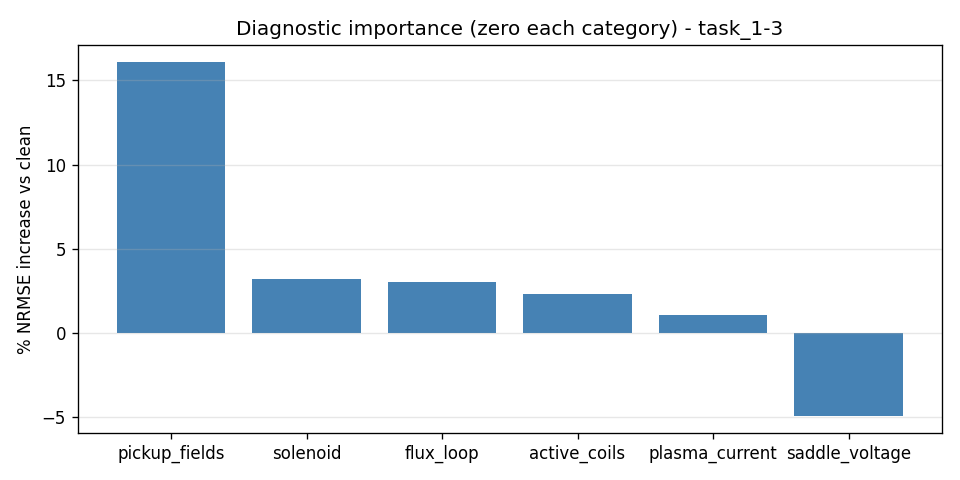
\includegraphics[width=\textwidth]{figures/mlp_signal_importance.png}\caption{\mlp{}}\end{subfigure}\hfill
\begin{subfigure}{0.48\textwidth}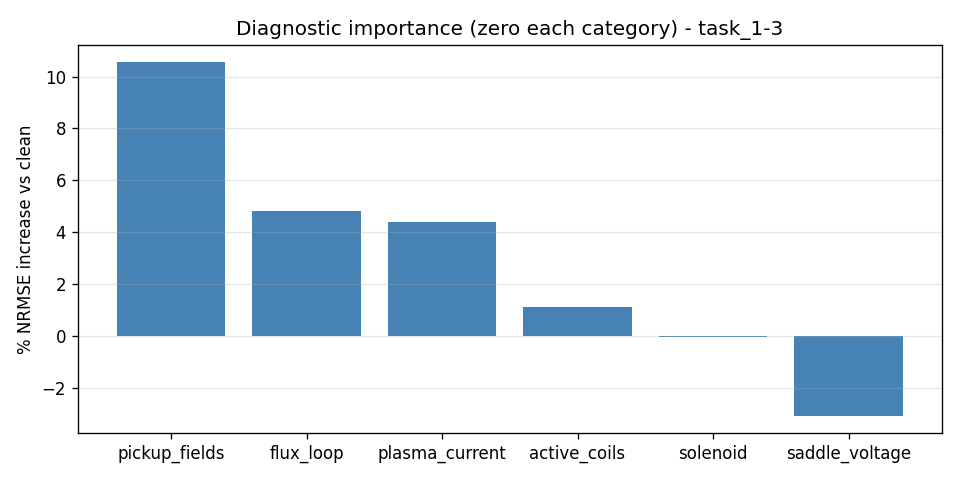
\includegraphics[width=\textwidth]{figures/lstm_signal_importance.png}\caption{\lstm{}}\end{subfigure}
\caption{Diagnostic importance: NRMSE change (\%) when a sensor category is zeroed.}
\label{fig:imp}
\end{figure}

% ------------------------------------------------------------------ module 3
\section{Module 3: sensor criticality and minimal sensor set}\label{sec:m3}
Each of the eight branches is removed in turn (zero-filled, mask set), and the change in boundary error in centimetres ranks its
criticality. A greedy backward elimination then removes the least critical branches while the boundary error stays below the
$2.0$\,cm tolerance.

\begin{table}[H]
\centering
\caption{Branch criticality (35 windows): boundary error with the branch lost, and change from the clean error (\CleanBndMLP\,cm MLP, \CleanBndLSTM\,cm LSTM).}
\label{tab:crit}
\small
\begin{tabular}{@{}lrcccc@{}}
\toprule
 & & \multicolumn{2}{c}{\mlp} & \multicolumn{2}{c}{\lstm} \\
\cmidrule(lr){3-4}\cmidrule(lr){5-6}
Branch & Probes & Error & Shift & Error & Shift \\
\midrule
\CritTable
\bottomrule
\end{tabular}
\end{table}

\begin{figure}[H]
\centering
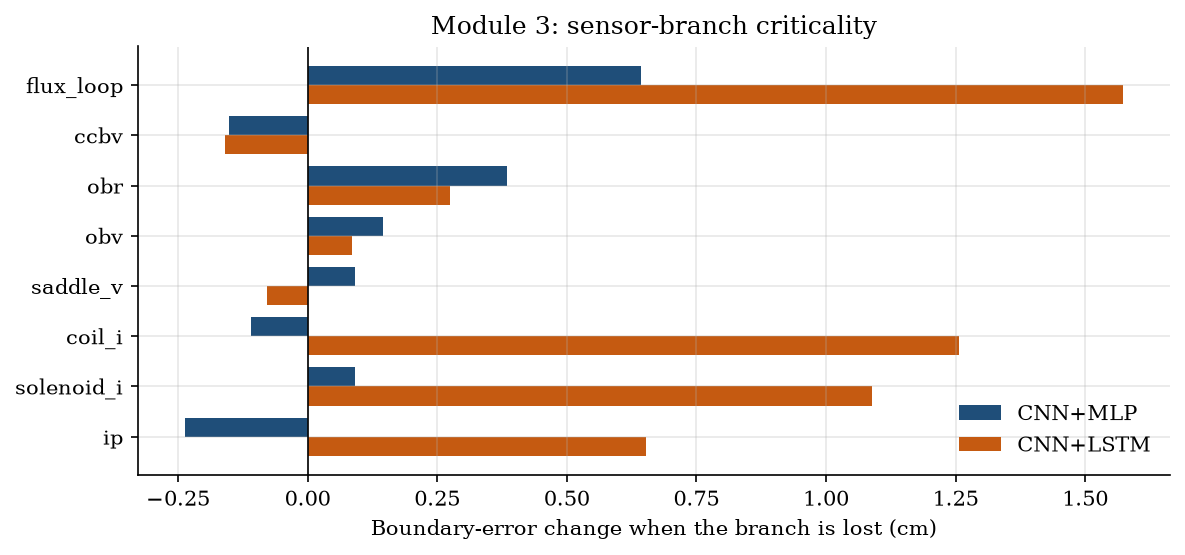
\includegraphics[width=0.8\textwidth]{figures/cmp_criticality.png}
\caption{Boundary-error shift when each branch is lost. Negative values mean the model does slightly better without that branch.}
\end{figure}

\paragraph{Findings.} The two models depend on different inputs: the LSTM relies most on the flux loops ($+1.6$\,cm), the coil currents
($+1.3$\,cm) and the solenoid current ($+1.1$\,cm), the MLP mostly on the flux loops ($+0.6$\,cm) and the outboard pickup probes. Because
the clean boundary error of both models already exceeds 2\,cm, elimination cannot start: \textbf{the minimal sensor set is the full
set of 115 probes for both models}, and every branch is classed Tier~1. The claim of pruning 47 probes to 25 is therefore \emph{not}
supported by these runs. The per-branch shifts are small ($|\Delta|<1.6$\,cm) compared with the 35-window noise.

\begin{figure}[H]
\centering
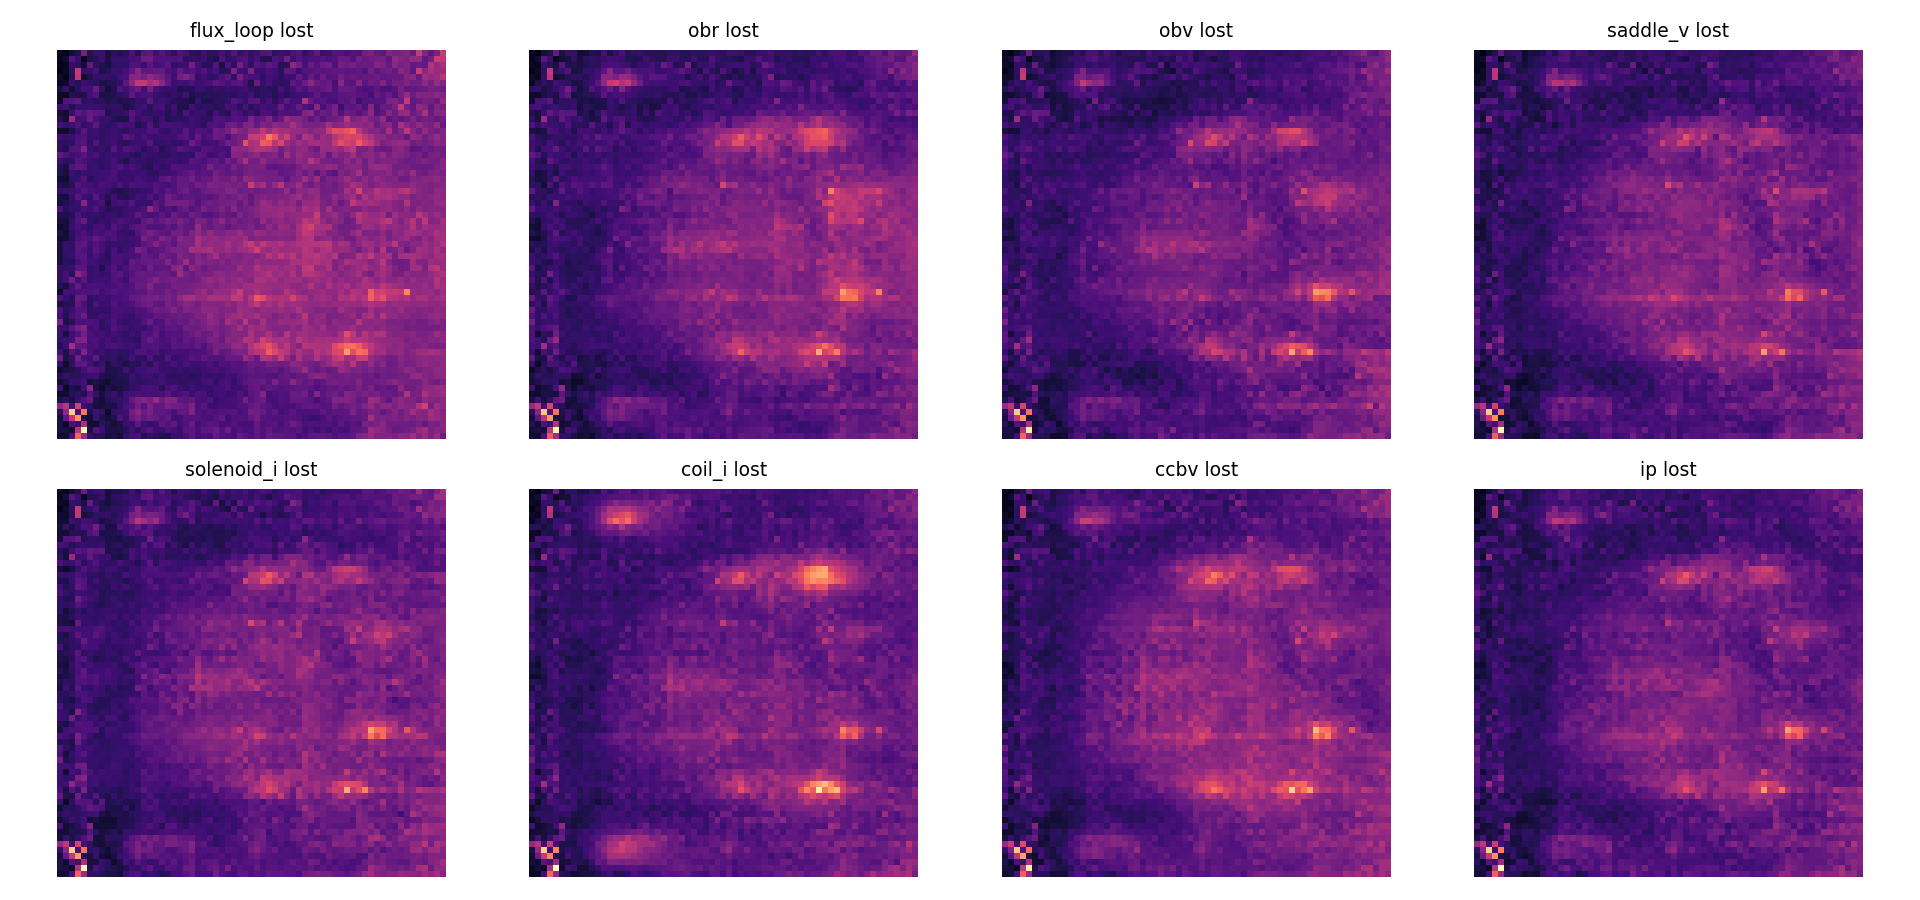
\includegraphics[width=0.95\textwidth]{figures/mlp_spatial_error_propagation_heatmaps.png}\\[4pt]
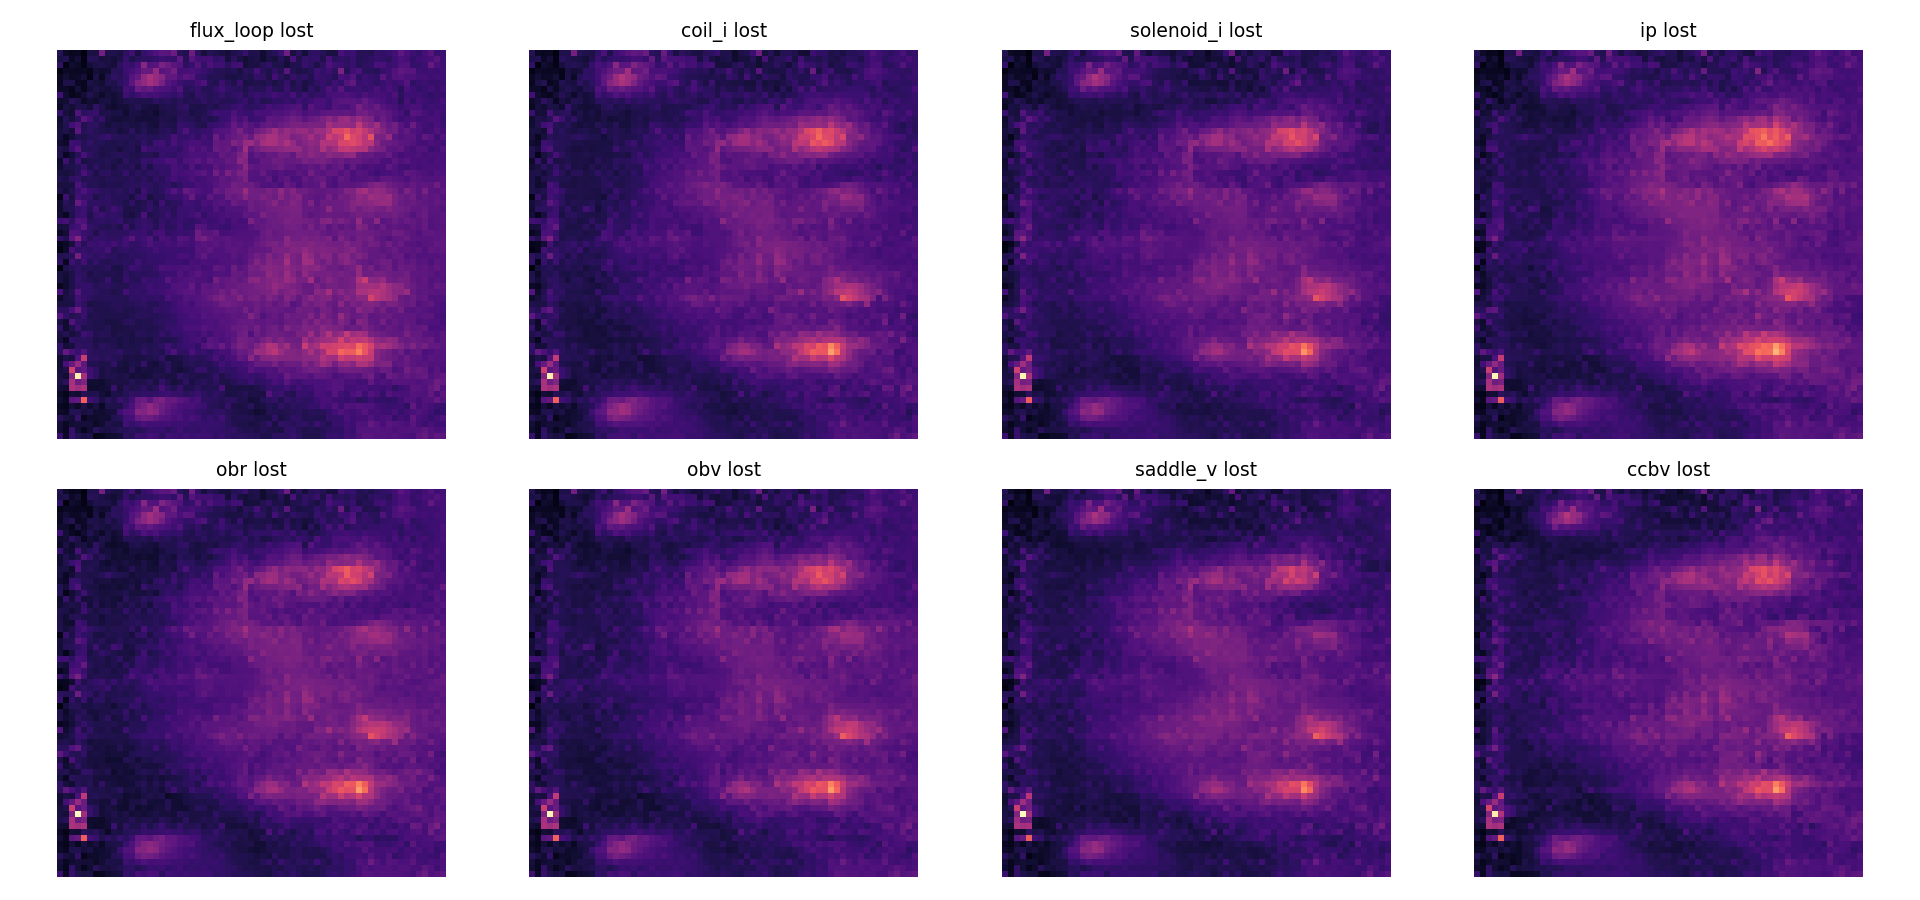
\includegraphics[width=0.95\textwidth]{figures/lstm_spatial_error_propagation_heatmaps.png}
\caption{Spatial propagation of the reconstruction error when a branch is lost: \mlp{} (top) and \lstm{} (bottom).
The elimination curve itself is a single point for both models (full set, above tolerance), so it is not plotted.}
\end{figure}

% ------------------------------------------------------------------ module 4
\section{Module 4: adaptive mitigation with a conformal gauge}\label{sec:m4}
The ``brain'' has three stages: a \emph{detector} (dead or stuck channels, saturation, impulse spikes, gaps); a \emph{router} that sends
transient faults to forward-fill, redundant probes to spatial neighbour regression, and critical or multi-sensor faults to the failure-aware
network with the mask set; and a \emph{conformal gauge} that adds a calibrated margin $\delta$ to the boundary estimate. $\delta$ is the 95th
percentile of the boundary error on validation windows (\NcalMLP{} calibration windows for the MLP, \NcalLSTM{} for the LSTM), and a
window is alarmed when the clearance minus $\delta$ falls below 5\,cm.

\begin{table}[H]
\centering
\caption{Module 4 on 35 test windows per scenario. Boundary error in cm for the bare model on zero-filled damage and with the brain.
False and missed alarms in \% as bare / brain / conservative (brain plus conformal margin). Last column: mean loop latency in ms.}
\label{tab:mit}
\small
\begin{tabular}{@{}llrrccr@{}}
\toprule
Model & Scenario & Bare & Brain & False (\%) & Missed (\%) & ms \\
\midrule
\MitTable
\bottomrule
\end{tabular}
\end{table}

\begin{figure}[H]
\centering
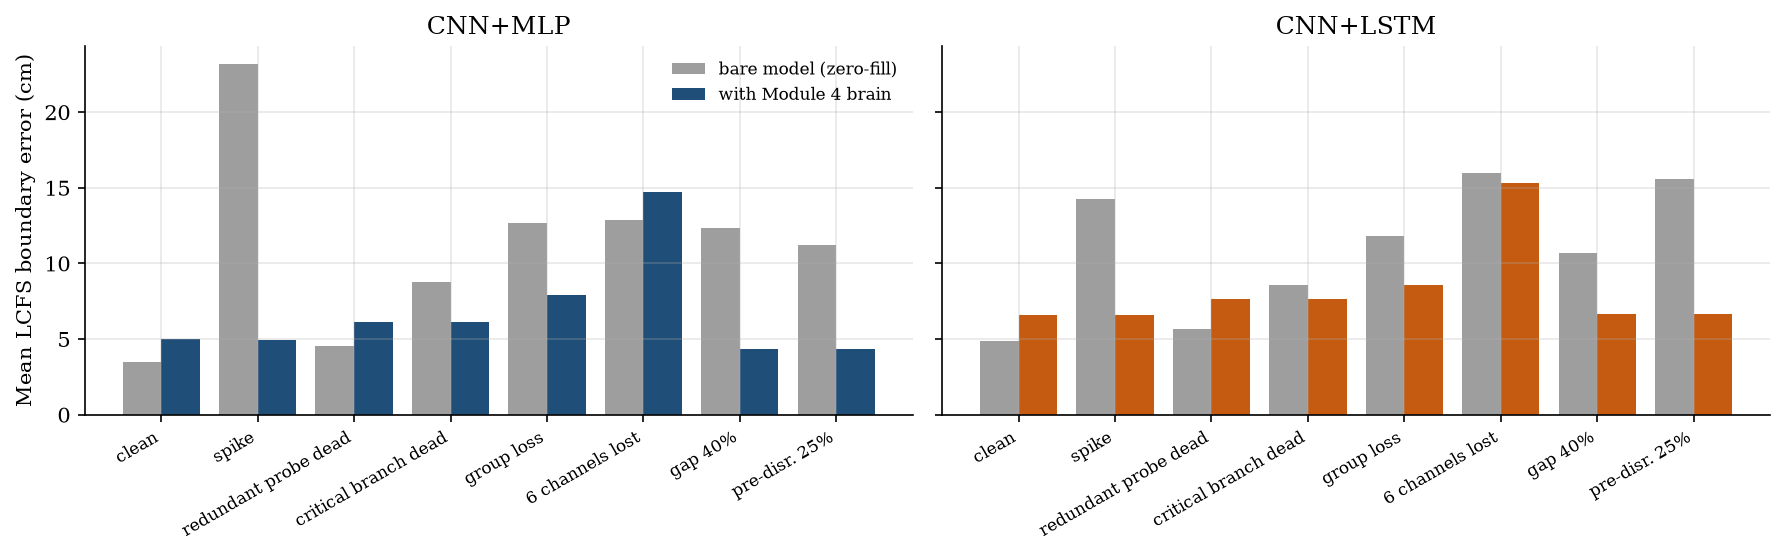
\includegraphics[width=\textwidth]{figures/cmp_mitigation.png}
\caption{Boundary error without (grey) and with (coloured) the mitigation brain.}
\end{figure}

\paragraph{Findings.}
\begin{itemize}
  \item \textbf{It helps where the fault is transient or structured.} Boundary error falls on spikes (MLP 23.2$\to$4.9\,cm, LSTM 14.3$\to$6.6),
        temporal gaps (12.4$\to$4.3 and 10.7$\to$6.7), pre-disruption windows (11.2$\to$4.4 and 15.6$\to$6.7) and group loss.
  \item \textbf{It hurts on healthy input and on large multi-channel loss.} Routing nearly every clean window to the failure-aware
        network raises clean error (3.48$\to$4.99\,cm MLP, 4.87$\to$6.57\,cm LSTM), and 6-channel loss is unchanged or worse.
  \item \textbf{The gauge is too conservative to be useful.} The conformal radius is \DeltaMLP\,cm (MLP) and \DeltaLSTM\,cm (LSTM), far larger than
        the 5\,cm clearance threshold, so every healthy window is flagged (100\% false alarms in the brain and conservative columns).
  \item \textbf{Latency is $\approx$\LatMLP\,ms (MLP) and \LatLSTM\,ms (LSTM)} per loop, dominated by the model forward pass on two
        T4 GPUs, against a 5\,ms budget.
\end{itemize}
The design targets of 8.2\% false alarms and 2.1\,ms latency were \emph{not} reproduced. The failure is likely in the calibration
(boundary error on a grid-edge clearance proxy with outlier windows) rather than in the idea, but this has not been investigated.

% ------------------------------------------------------------------ limitations
\section{Limitations and how to quote these results}\label{sec:limits}
\begin{itemize}
  \item \textbf{Different training loops.} The LSTM and the old MLP use the step loop; the MLP used for the robustness sweep (NRMSE
        \NRMSEmlp) is a newer epoch-trained run whose checkpoint is the one tested. Robustness comparisons are therefore between
        models of slightly different provenance.
  \item \textbf{No plain-model sweep on this engine.} We have not run a non-failure-aware baseline through the same 63 passes, so the
        \emph{benefit} of failure-aware training is not proven here. An earlier plain-MLP sweep (clean NRMSE 0.142, in \texttt{results/robustness}) used a different engine.
  \item \textbf{Single seed, single split.} No confidence intervals across seeds; differences of a few percent in NRMSE may be within seed noise.
  \item \textbf{Small physics samples.} Modules 1, 3 and 4 use 35 windows per pass; X-point and wall-clearance metrics are unreliable.
  \item \textbf{Boundary-overlay figure.} A purely visual overlay at the 35\% flux level of the true field; for two-lobed fields it can trace the coil
        regions rather than the plasma boundary, so its centimetre offsets should not be quoted.
  \item \textbf{Older claims.} The figures in the repository's design document (47 to 25 probes, 75.5\% to 8.2\% false alarms, 2.1\,ms) are
        not reproduced by these runs and should be replaced by the measured values above.
\end{itemize}

\section{Reproducibility}
Training and robustness each ran as a Kaggle kernel on 2$\times$T4.
\begin{itemize}
  \item Training: kernel \texttt{tokamark-train-lstm-fa} (CNN+LSTM, 190\,min), built by \path{scripts/build_lstm_kernel.py} from \path{src/pipeline.py}.
  \item Robustness, Modules 1, 3, 4: kernel \texttt{tokamark-robust-lstm-fa}, built by \path{scripts/build_lstm_robust_kernel.py} from \path{src/study/}.
  \item This document: run \path{report/build_report_assets.py}, then compile \path{report/report.tex} (paths relative to \path{cnn_mlp/}).
\end{itemize}

\appendix
\section{Full zero-fill sweep}\label{app:sweep}
\begin{table}[H]
\centering
\caption{NRMSE and robustness score for every setting (zero-fill). Format: scenario$|$severity.}
\small
\begin{tabular}{@{}lcccc@{}}
\toprule
 & \multicolumn{2}{c}{NRMSE} & \multicolumn{2}{c}{RS} \\
\cmidrule(lr){2-3}\cmidrule(lr){4-5}
Setting & \mlp & \lstm & \mlp & \lstm \\
\midrule
\SweepTable
\bottomrule
\end{tabular}
\end{table}

\end{document}
